\section{Simulations Experiments}
\subsection{Scenario Calibration}
In order to calibrate the simulator parameters, the following range of values were used:
\begin{itemize}
	\item \textbf{Number of Couples Tx-Rx}: [5, 30]
	\item \textbf{Number of Channels C} : [6, 100] (Resource Blocks in LTE for different Frequencies)
	\item \textbf{Mean Inter-arrival Time (1/lambda)}: [25ms, 500ms]   
	\item \textbf{Time-slot duration $T_{slot}$}: 0.5 ms (Timeslot duration in LTE)
	\item \textbf{Time Threshold}: [5ms, 50ms] 
	\item \textbf{Send Probability p}: [0.2, 0.5] 
\end{itemize}

\subsection{Calibration of Warm-Up Period and Simulation duration}
For calibrating the warm-up different simulation were made (with the factors range in the latter paragraph) with 10 repetition each. 
The worst case in terms of convergence time was encountered with the \textbf{mean throughput} with N = 5, C = 6, $\dfrac{1}{\lambda}$ = 500ms, p = 0.5:
\begin{figure}[H]
	\centering
	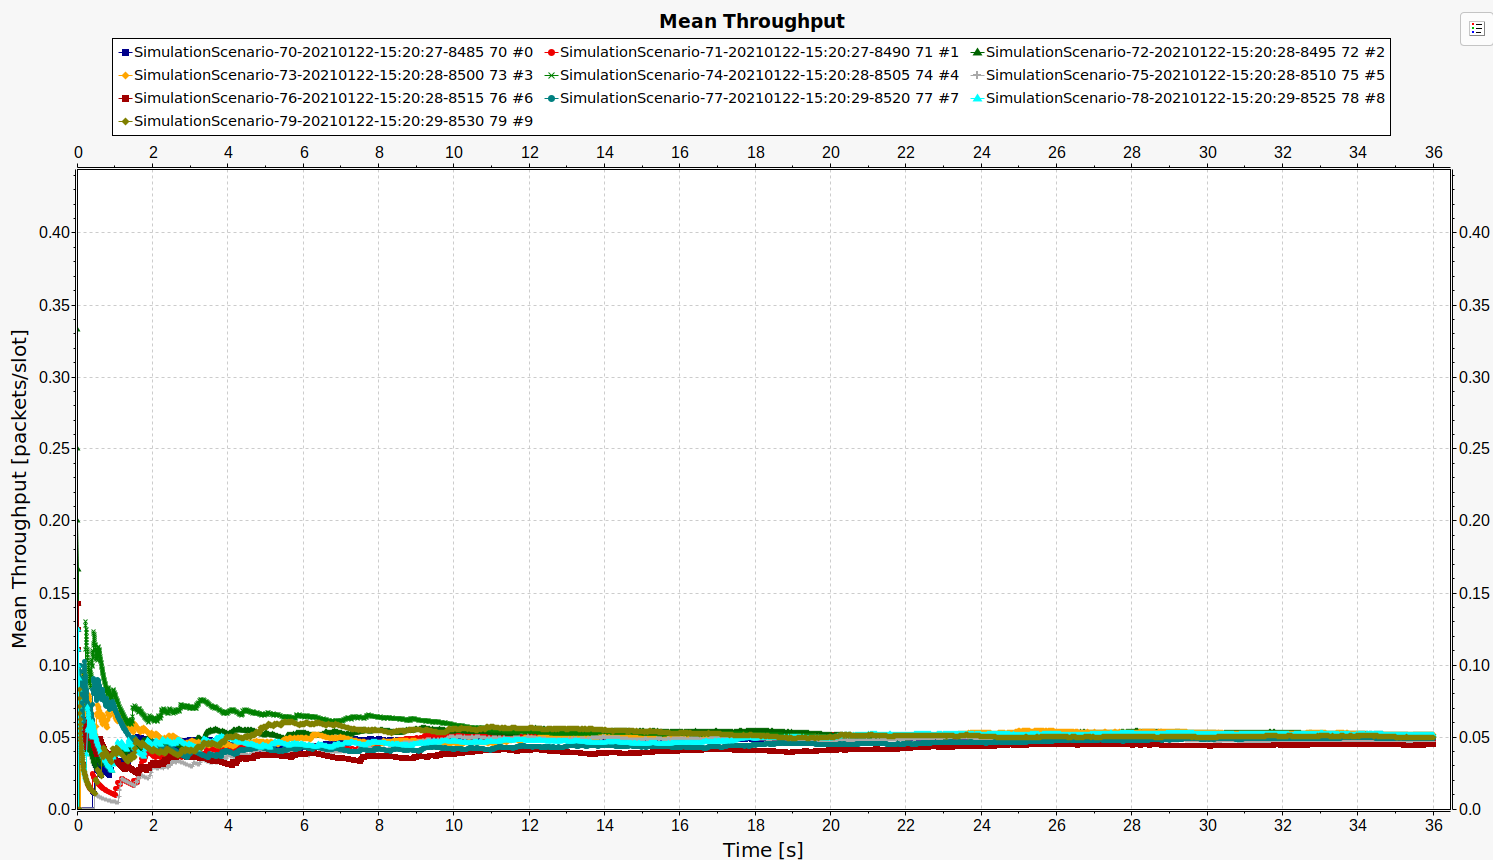
\includegraphics[width=\textwidth]{img/WorstCaseWarmUp.png}
	\caption{Worst Case Warm-up}
	\label {img: warmUp}
\end{figure}  
\noindent\textbf{A warm-up period of 10s was chosen}.
For what concerns the simulation duration was made a trade-off between the memory consumption and the length of the simulation itself. This was done because there are not stochastic elements in the model (like a particular error probability with a low percentage) that will need a particular amount of time to be shown. Obviously the duration has to be greater than the warm-up duration. All things considered, \textbf{a simulation-duration of 100s was chose}

\subsection{Design of Experiments}
\subsection{Result Analysis}